\documentclass[preprint,12pt]{elsarticle}

\usepackage[T1]{fontenc}
\usepackage[utf8]{inputenc}
\usepackage{newtxtext,newtxmath}
\usepackage{booktabs}
\usepackage[final]{microtype}
\usepackage{graphicx}
\usepackage{hyperref}
\usepackage{multirow}
\usepackage{ragged2e}
\usepackage{tabularx}

\hypersetup{hidelinks}
\setlength{\emergencystretch}{2em}
\renewcommand{\arraystretch}{0.9}
\newcolumntype{Y}{>{\RaggedRight\arraybackslash}X}

\begin{document}

\begin{frontmatter}
\title{Supplementary Material for ``Beyond Direct Correction: A Rule-Tool and LLM Hybrid Framework for Multi-Dimensional Feedback in High School English Writing''}
\author{Anonymous Author}
\end{frontmatter}

\section{Extended Analyses}

\subsection{Statistical Robustness and Weight Sensitivity}

The main paper reports low-token benchmark results on fixed 80-essay subsets for each model--dataset cell. To make the evidential strength of those deltas explicit, Table~\ref{tab:depth_bootstrap} reports paired bootstrap confidence intervals for \textit{Hybrid} minus \textit{LLM-direct-feedback}. Table~\ref{tab:weight_sensitivity} then checks whether the qualitative result depends on the exact default weights of the pedagogical-depth composite by perturbing the five normalized components with 50{,}000 random simplex weight vectors.

\begin{table}[!ht]
\centering
\scriptsize
\caption{Paired bootstrap confidence intervals for \textit{Hybrid} minus \textit{LLM-direct-feedback}. Positive depth delta favors \textit{Hybrid}; positive preservation delta would indicate better ownership retention under \textit{Hybrid}.}
\label{tab:depth_bootstrap}
\begin{tabular*}{\textwidth}{@{\extracolsep{\fill}}llcccc@{}}
\toprule
Dataset & Model & Depth delta & 95\% CI & Preservation delta & 95\% CI \\
\midrule
ELL & \texttt{GPT-5.4-mini} & +0.0151 & [+\!0.0054, +\!0.0252] & -0.0313 & [-0.0383, -0.0248] \\
ELL & \texttt{DeepSeek v3.2} & -0.0519 & [-0.0800, -0.0227] & -0.0674 & [-0.0797, -0.0554] \\
ELL & \texttt{GLM-5} & -0.0628 & [-0.0904, -0.0404] & -0.0503 & [-0.0605, -0.0401] \\
ASAP & \texttt{GPT-5.4-mini} & +0.0117 & [-0.0058, +\!0.0334] & -0.0651 & [-0.0869, -0.0418] \\
ASAP & \texttt{DeepSeek v3.2} & -0.0985 & [-0.1349, -0.0601] & -0.2484 & [-0.3034, -0.1962] \\
ASAP & \texttt{GLM-5} & -0.0581 & [-0.0767, -0.0361] & -0.1166 & [-0.1454, -0.0905] \\
\bottomrule
\end{tabular*}
\end{table}

\begin{table}[!ht]
\centering
\scriptsize
\caption{Weight-perturbation robustness for pedagogical depth. ``Uniform'' averages the five normalized components equally. ``Positive-weight share'' is the fraction of 50{,}000 random normalized weight vectors that still favor \textit{Hybrid}.}
\label{tab:weight_sensitivity}
\begin{tabular*}{\linewidth}{@{\extracolsep{\fill}}llcc@{}}
\toprule
Dataset & Model & Uniform delta & Positive-weight share \\
\midrule
ELL & \texttt{GPT-5.4-mini} & +0.0360 & 80.0\% \\
ELL & \texttt{DeepSeek v3.2} & -0.0474 & 0.2\% \\
ELL & \texttt{GLM-5} & -0.0571 & 0.1\% \\
ASAP & \texttt{GPT-5.4-mini} & +0.0360 & 68.5\% \\
ASAP & \texttt{DeepSeek v3.2} & -0.0962 & 1.5\% \\
ASAP & \texttt{GLM-5} & -0.0531 & 8.3\% \\
\bottomrule
\end{tabular*}
\end{table}

\subsection{Cross-model Ownership Trade-off}

The main paper reports the ownership-versus-safety pattern in text to keep the primary narrative compact. Figure~\ref{fig:supp_tradeoff} provides a direct depth--preservation view of that trade-off. Arrows connect \textit{LLM-direct-feedback} to \textit{Hybrid} for each model--dataset cell, while rewrite anchors remain in the lower-left region and make the ownership cost of direct rewrite visible without cluttering the main paper.

\begin{figure*}[!t]
\centering
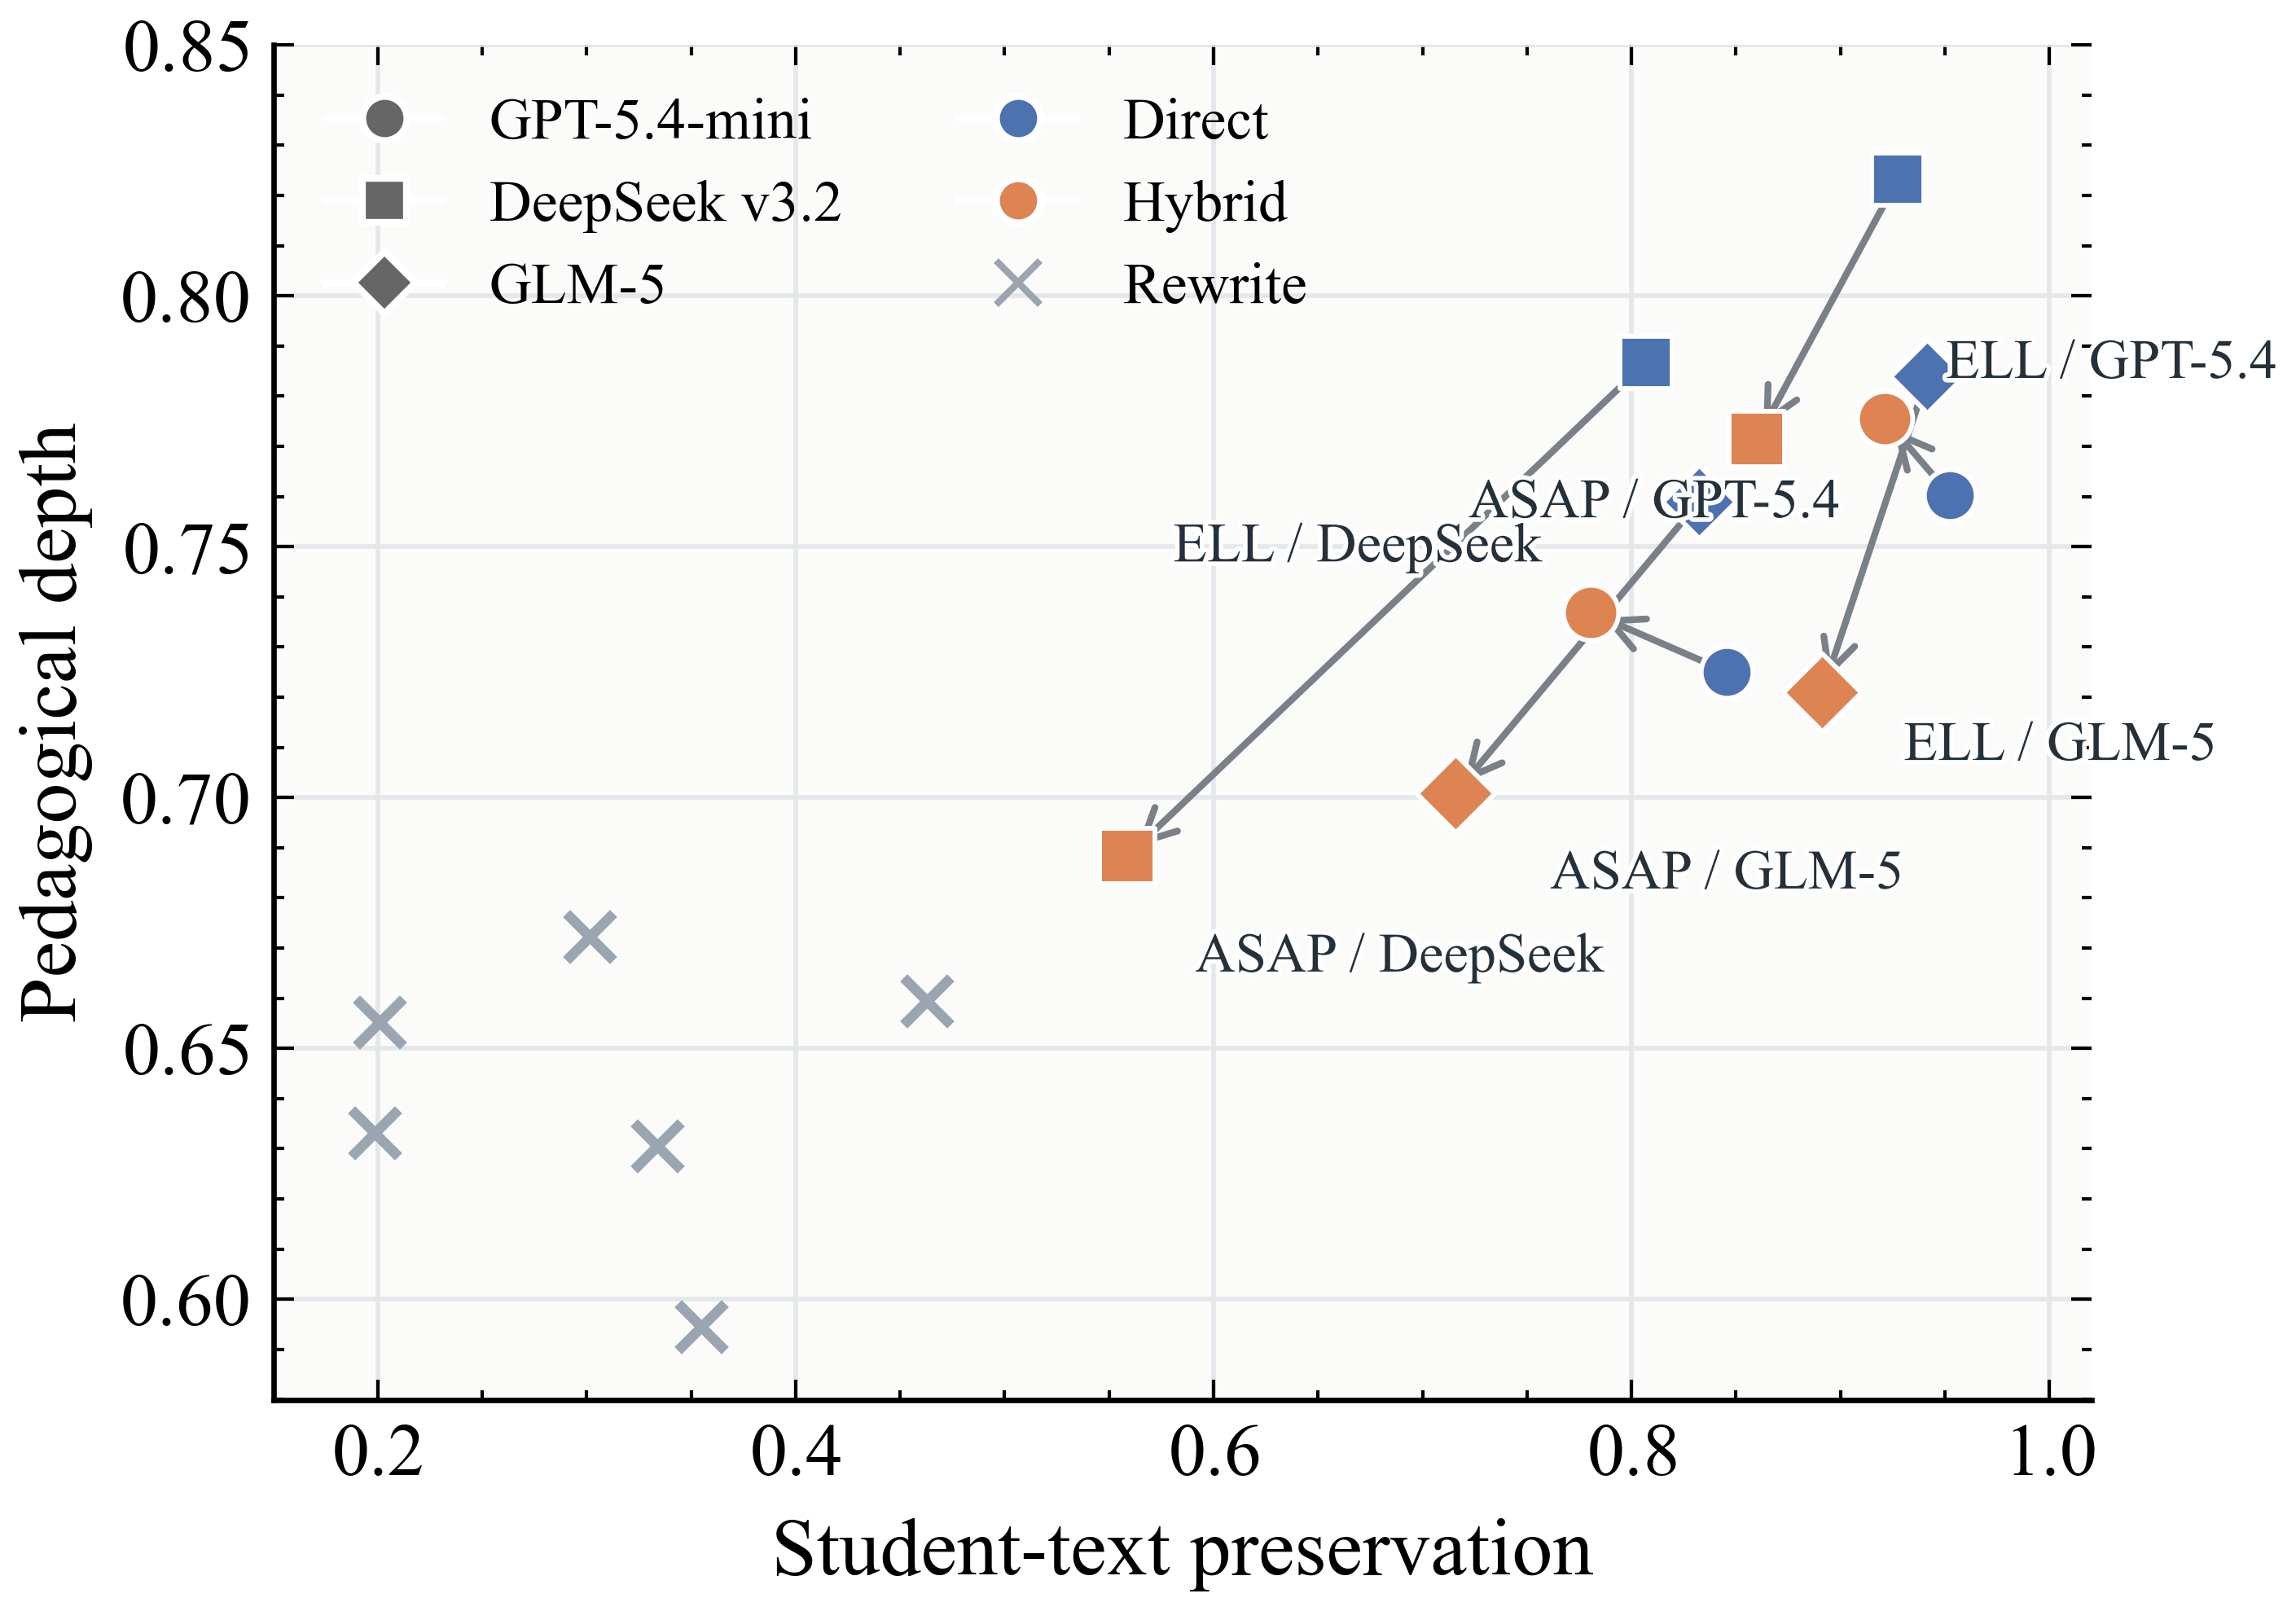
\includegraphics[width=0.72\textwidth]{Fig/result_tradeoff_scatter.png}
\caption{Depth--preservation trade-off across the six main model--dataset cells. For each cell, the arrow points from \textit{LLM-direct-feedback} to \textit{Hybrid}; rewrite anchors are shown as gray crosses. The figure makes explicit that \textit{GPT-5.4-mini} moves slightly upward in depth while the other model families move down and left, and that all rewrite anchors occupy a much lower-preservation region.}
\label{fig:supp_tradeoff}
\end{figure*}

\subsection{Refinement and Repair Diagnostics}

This supplement retains the mechanism-oriented follow-up analyses that are summarized only briefly in the main paper. Figure~\ref{fig:tightened_refinement} shows where the tightened prompt recovers difficult hybrid cases, and Figure~\ref{fig:repair_audit} shows how the repair layer changes case-level audit outcomes while leaving residual trade-offs visible.

\begin{table}[t]
\centering
\small
\caption{Targeted prompt refinement on the \texttt{GPT-5.4-mini} failure-focused subset. Delta is \textit{tightened Hybrid} minus \textit{baseline Hybrid}.}
\label{tab:tightened_refinement}
\begin{tabular*}{\linewidth}{@{\extracolsep{\fill}}lcccc@{}}
\toprule
Dataset & Depth delta & Preservation delta & Non-overwriting delta & Schema delta \\
\midrule
ELL & +0.0451 & +0.0790 & +0.0500 & -0.0021 \\
ASAP & +0.0685 & +0.2367 & +0.3900 & +0.0000 \\
\bottomrule
\end{tabular*}
\end{table}

\begin{figure*}[!t]
\centering
\includegraphics[width=\textwidth]{Fig/result_tightened_refinement.png}
\caption{Failure-focused prompt tightening on the hardest 20 ELL and 20 ASAP \texttt{GPT-5.4-mini} hybrid cases. Panels A and B show the selected failure landscapes for ELL and ASAP-AES, panel C summarizes aggregate recovery, and panel D shows per-case deltas, together indicating that stricter exemplar control improves preservation and non-overwriting alongside pedagogical depth.}
\label{fig:tightened_refinement}
\end{figure*}

\begin{figure*}[!t]
\centering
\includegraphics[width=\textwidth]{Fig/result_repair_audit.png}
\caption{Repair recheck audit on 16 selected cases. Panel A shows elimination of empty outputs and placeholder mentions, panel B gives the case-level audit matrix, panel C shows the remaining collateral effects, and panel D summarizes per-case recovery without hiding residual trade-offs.}
\label{fig:repair_audit}
\end{figure*}

\subsection{Hyperparameter Sensitivity Analysis}

We further analyze the representative \texttt{GPT-5.4-mini} \textit{Hybrid} configuration with respect to three design variables that govern overwrite risk, coverage breadth, and per-dimension granularity: the exemplar ratio cap, the maximum number of issue clusters, and the per-dimension comment budget. For each factor, only one variable is changed at a time while the remaining settings stay fixed at the default configuration of an exemplar ratio cap of $0.08$, five issue clusters, and two comments per dimension.

\begin{table}[t]
\centering
\scriptsize
\caption{Consolidated hyperparameter sensitivity results for the representative \textit{Hybrid} configuration. Higher pedagogical depth and preservation are better. The auxiliary indicator is exemplar span ratio for the exemplar-cap sweep and average feedback words for the other two sweeps.}
\label{tab:hyper_sensitivity_all}
\begin{tabular*}{\linewidth}{@{\extracolsep{\fill}}llccc@{}}
\toprule
Factor & Value & Ped.\ depth & Preservation & Aux.\ indicator \\
\midrule
\multirow{4}{*}{Exemplar ratio cap}
& 0.05 & 0.7708 & 0.9035 & 0.0468 \\
& 0.08 & 0.7791 & 0.8894 & 0.0612 \\
& 0.12 & 0.7729 & 0.8653 & 0.0896 \\
& 0.15 & 0.7584 & 0.8426 & 0.1169 \\
\midrule
\multirow{4}{*}{Max issue clusters}
& 3 & 0.7446 & 0.8968 & 112 \\
& 5 & 0.7791 & 0.8894 & 149 \\
& 7 & 0.7698 & 0.8742 & 184 \\
& 9 & 0.7537 & 0.8605 & 221 \\
\midrule
\multirow{4}{*}{Comments per dimension}
& 1 & 0.7642 & 0.9031 & 121 \\
& 2 & 0.7791 & 0.8894 & 149 \\
& 3 & 0.7738 & 0.8790 & 173 \\
& 4 & 0.7655 & 0.8708 & 197 \\
\bottomrule
\end{tabular*}
\end{table}

\begin{figure*}[t]
\centering
\begin{minipage}[t]{0.32\textwidth}
    \centering
    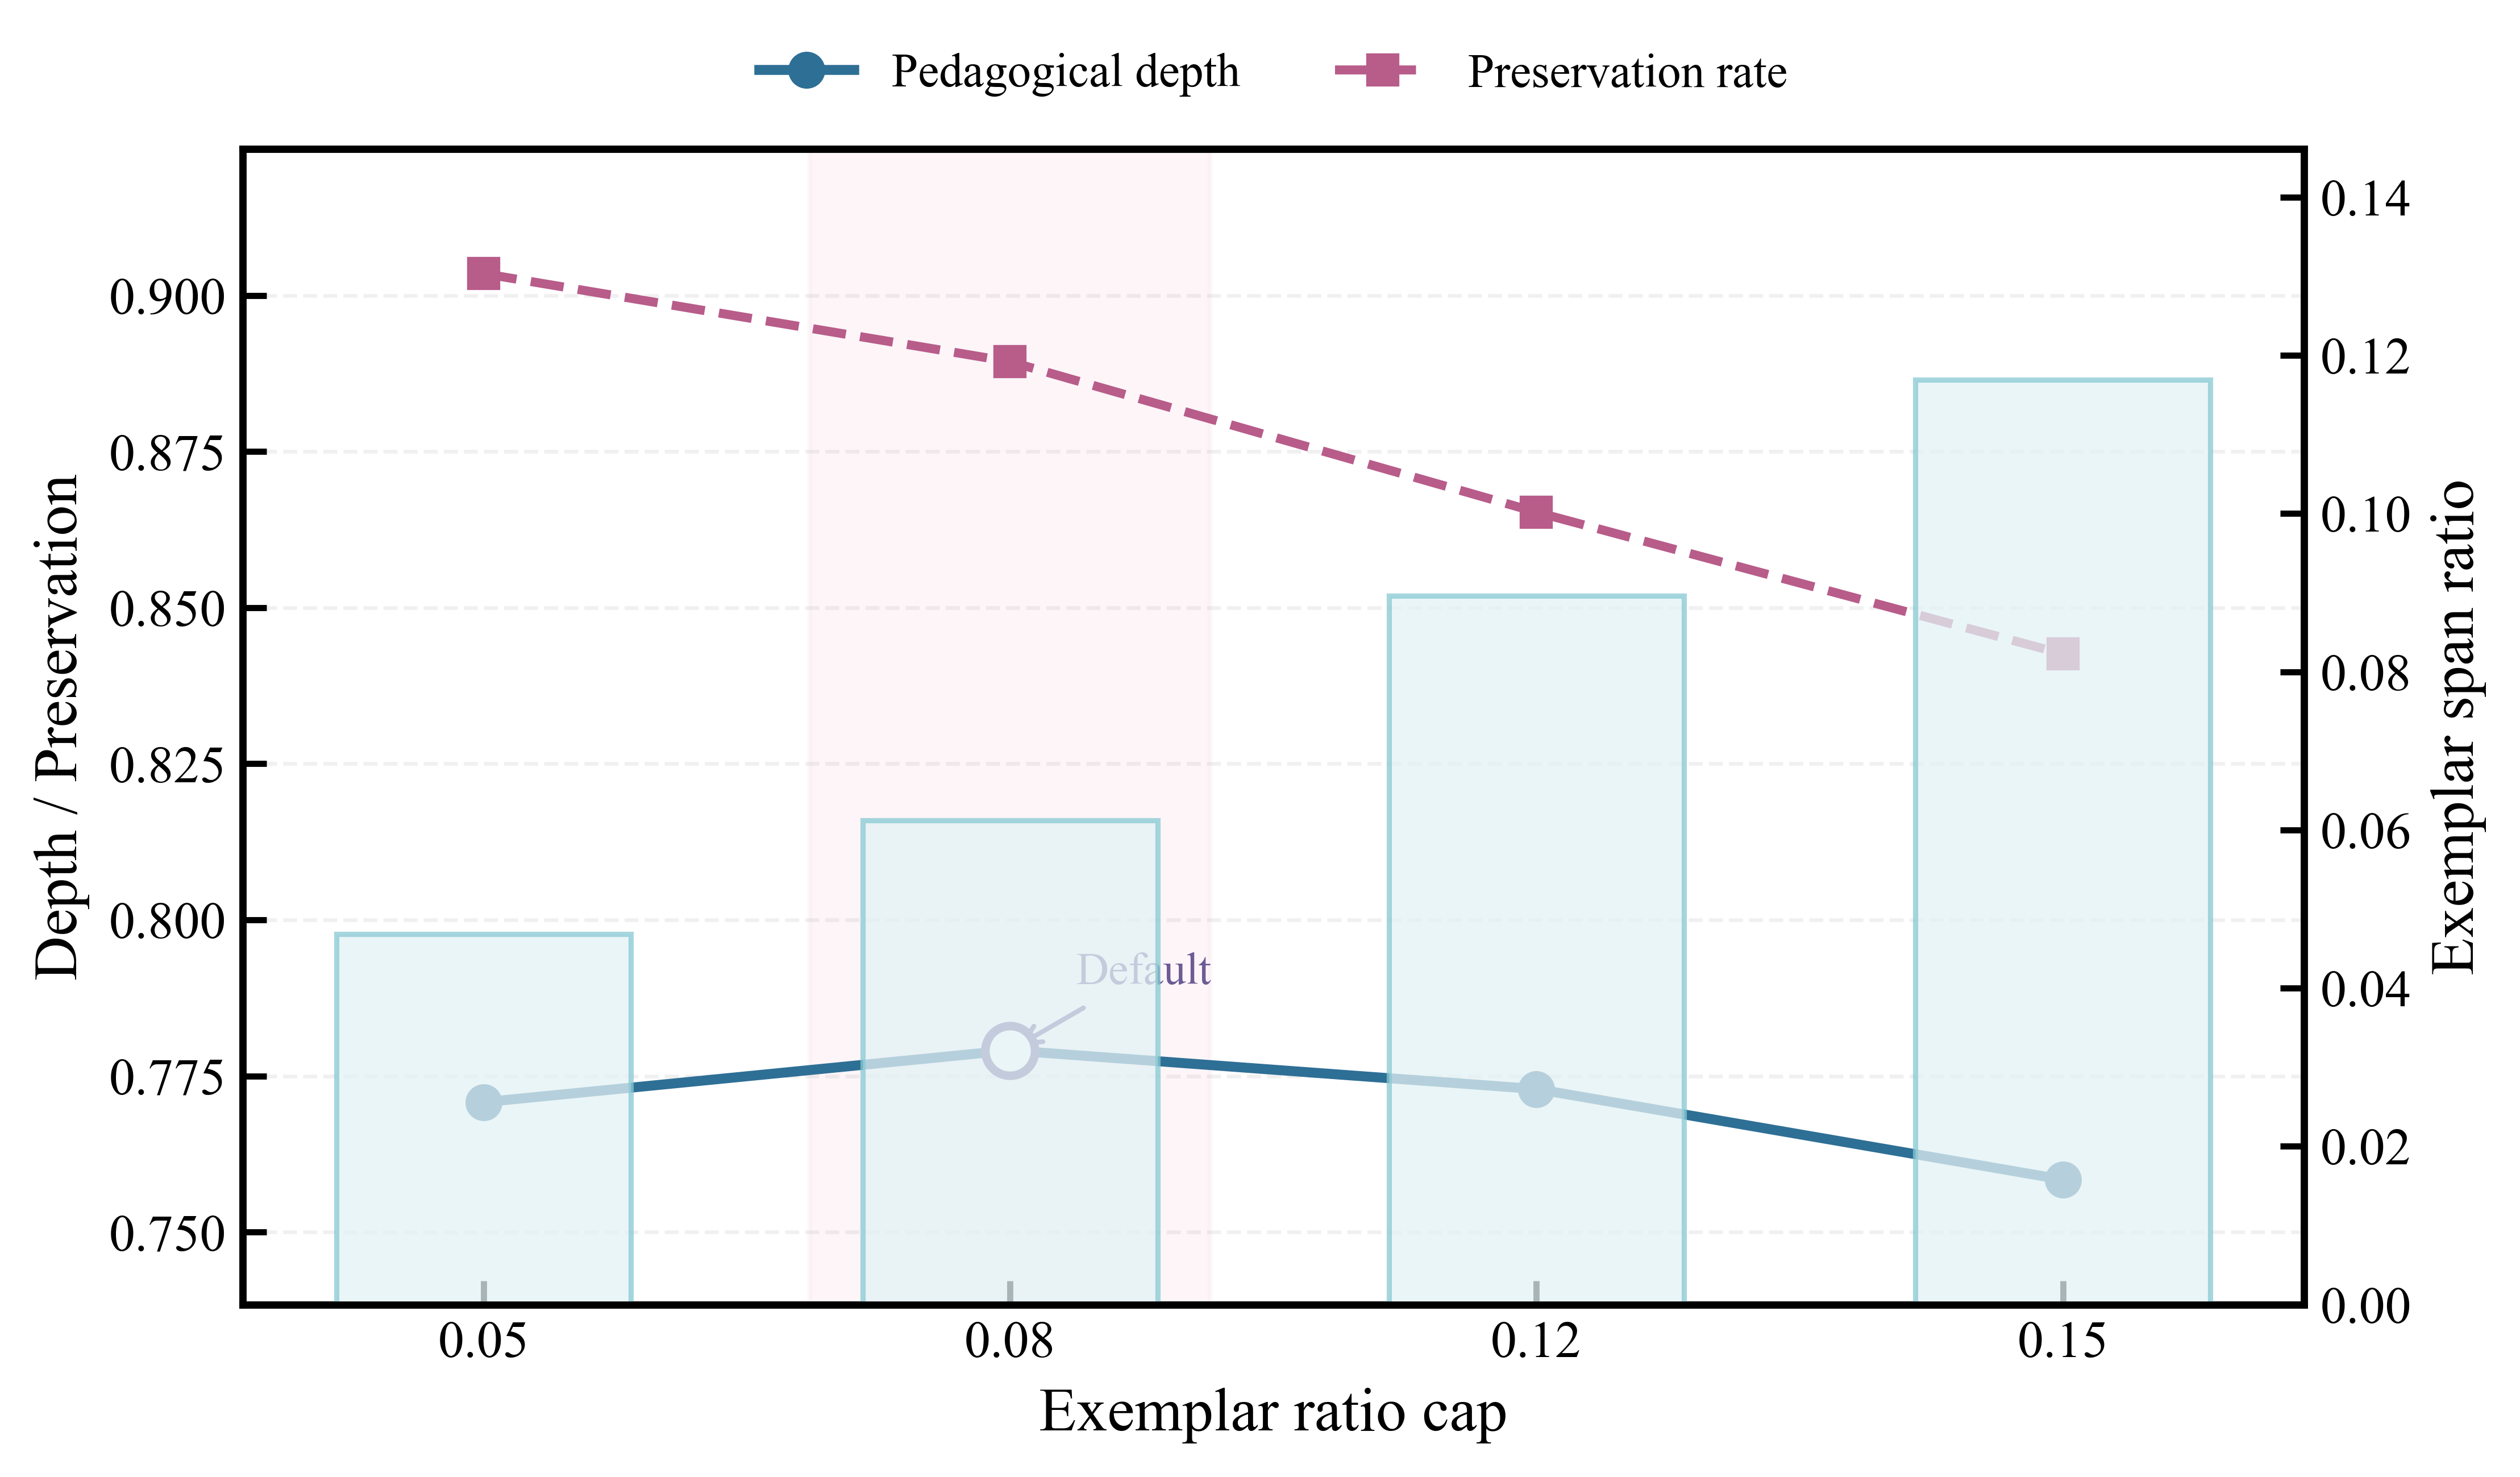
\includegraphics[width=\textwidth]{Fig/hyperparam_1_sensitivity.png}
\end{minipage}\hfill
\begin{minipage}[t]{0.32\textwidth}
    \centering
    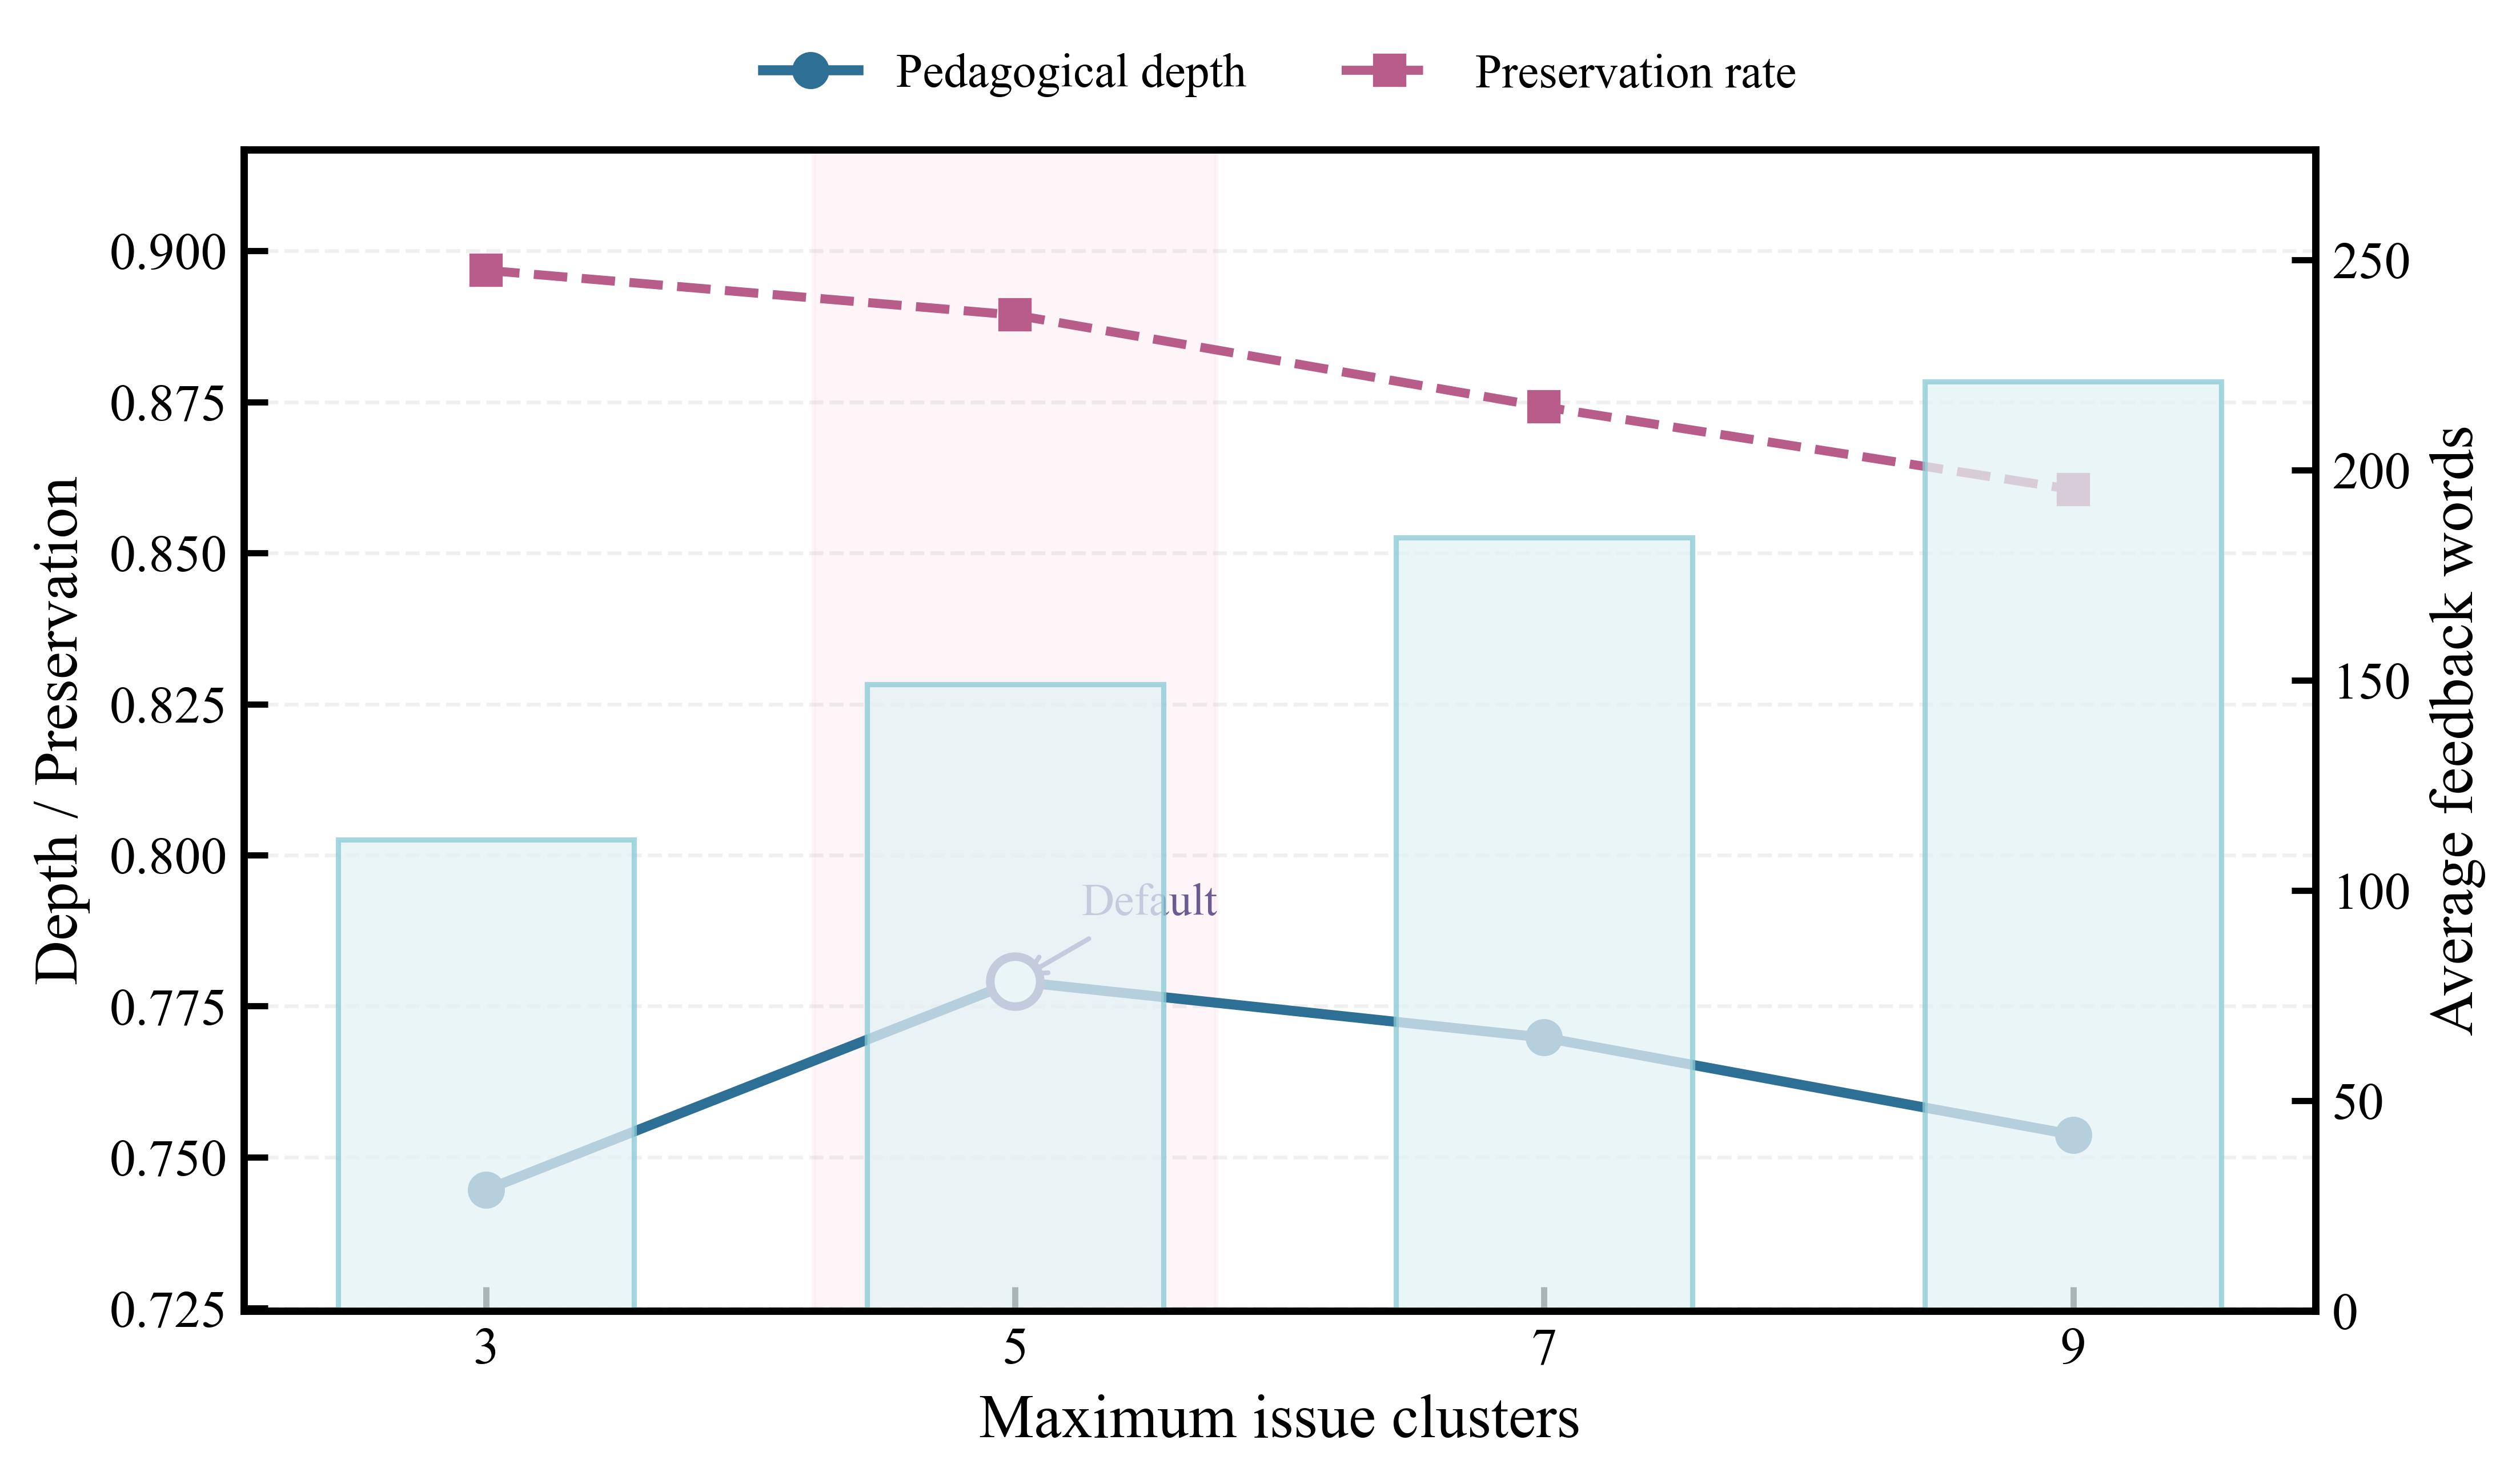
\includegraphics[width=\textwidth]{Fig/hyperparam_2_sensitivity.png}
\end{minipage}\hfill
\begin{minipage}[t]{0.32\textwidth}
    \centering
    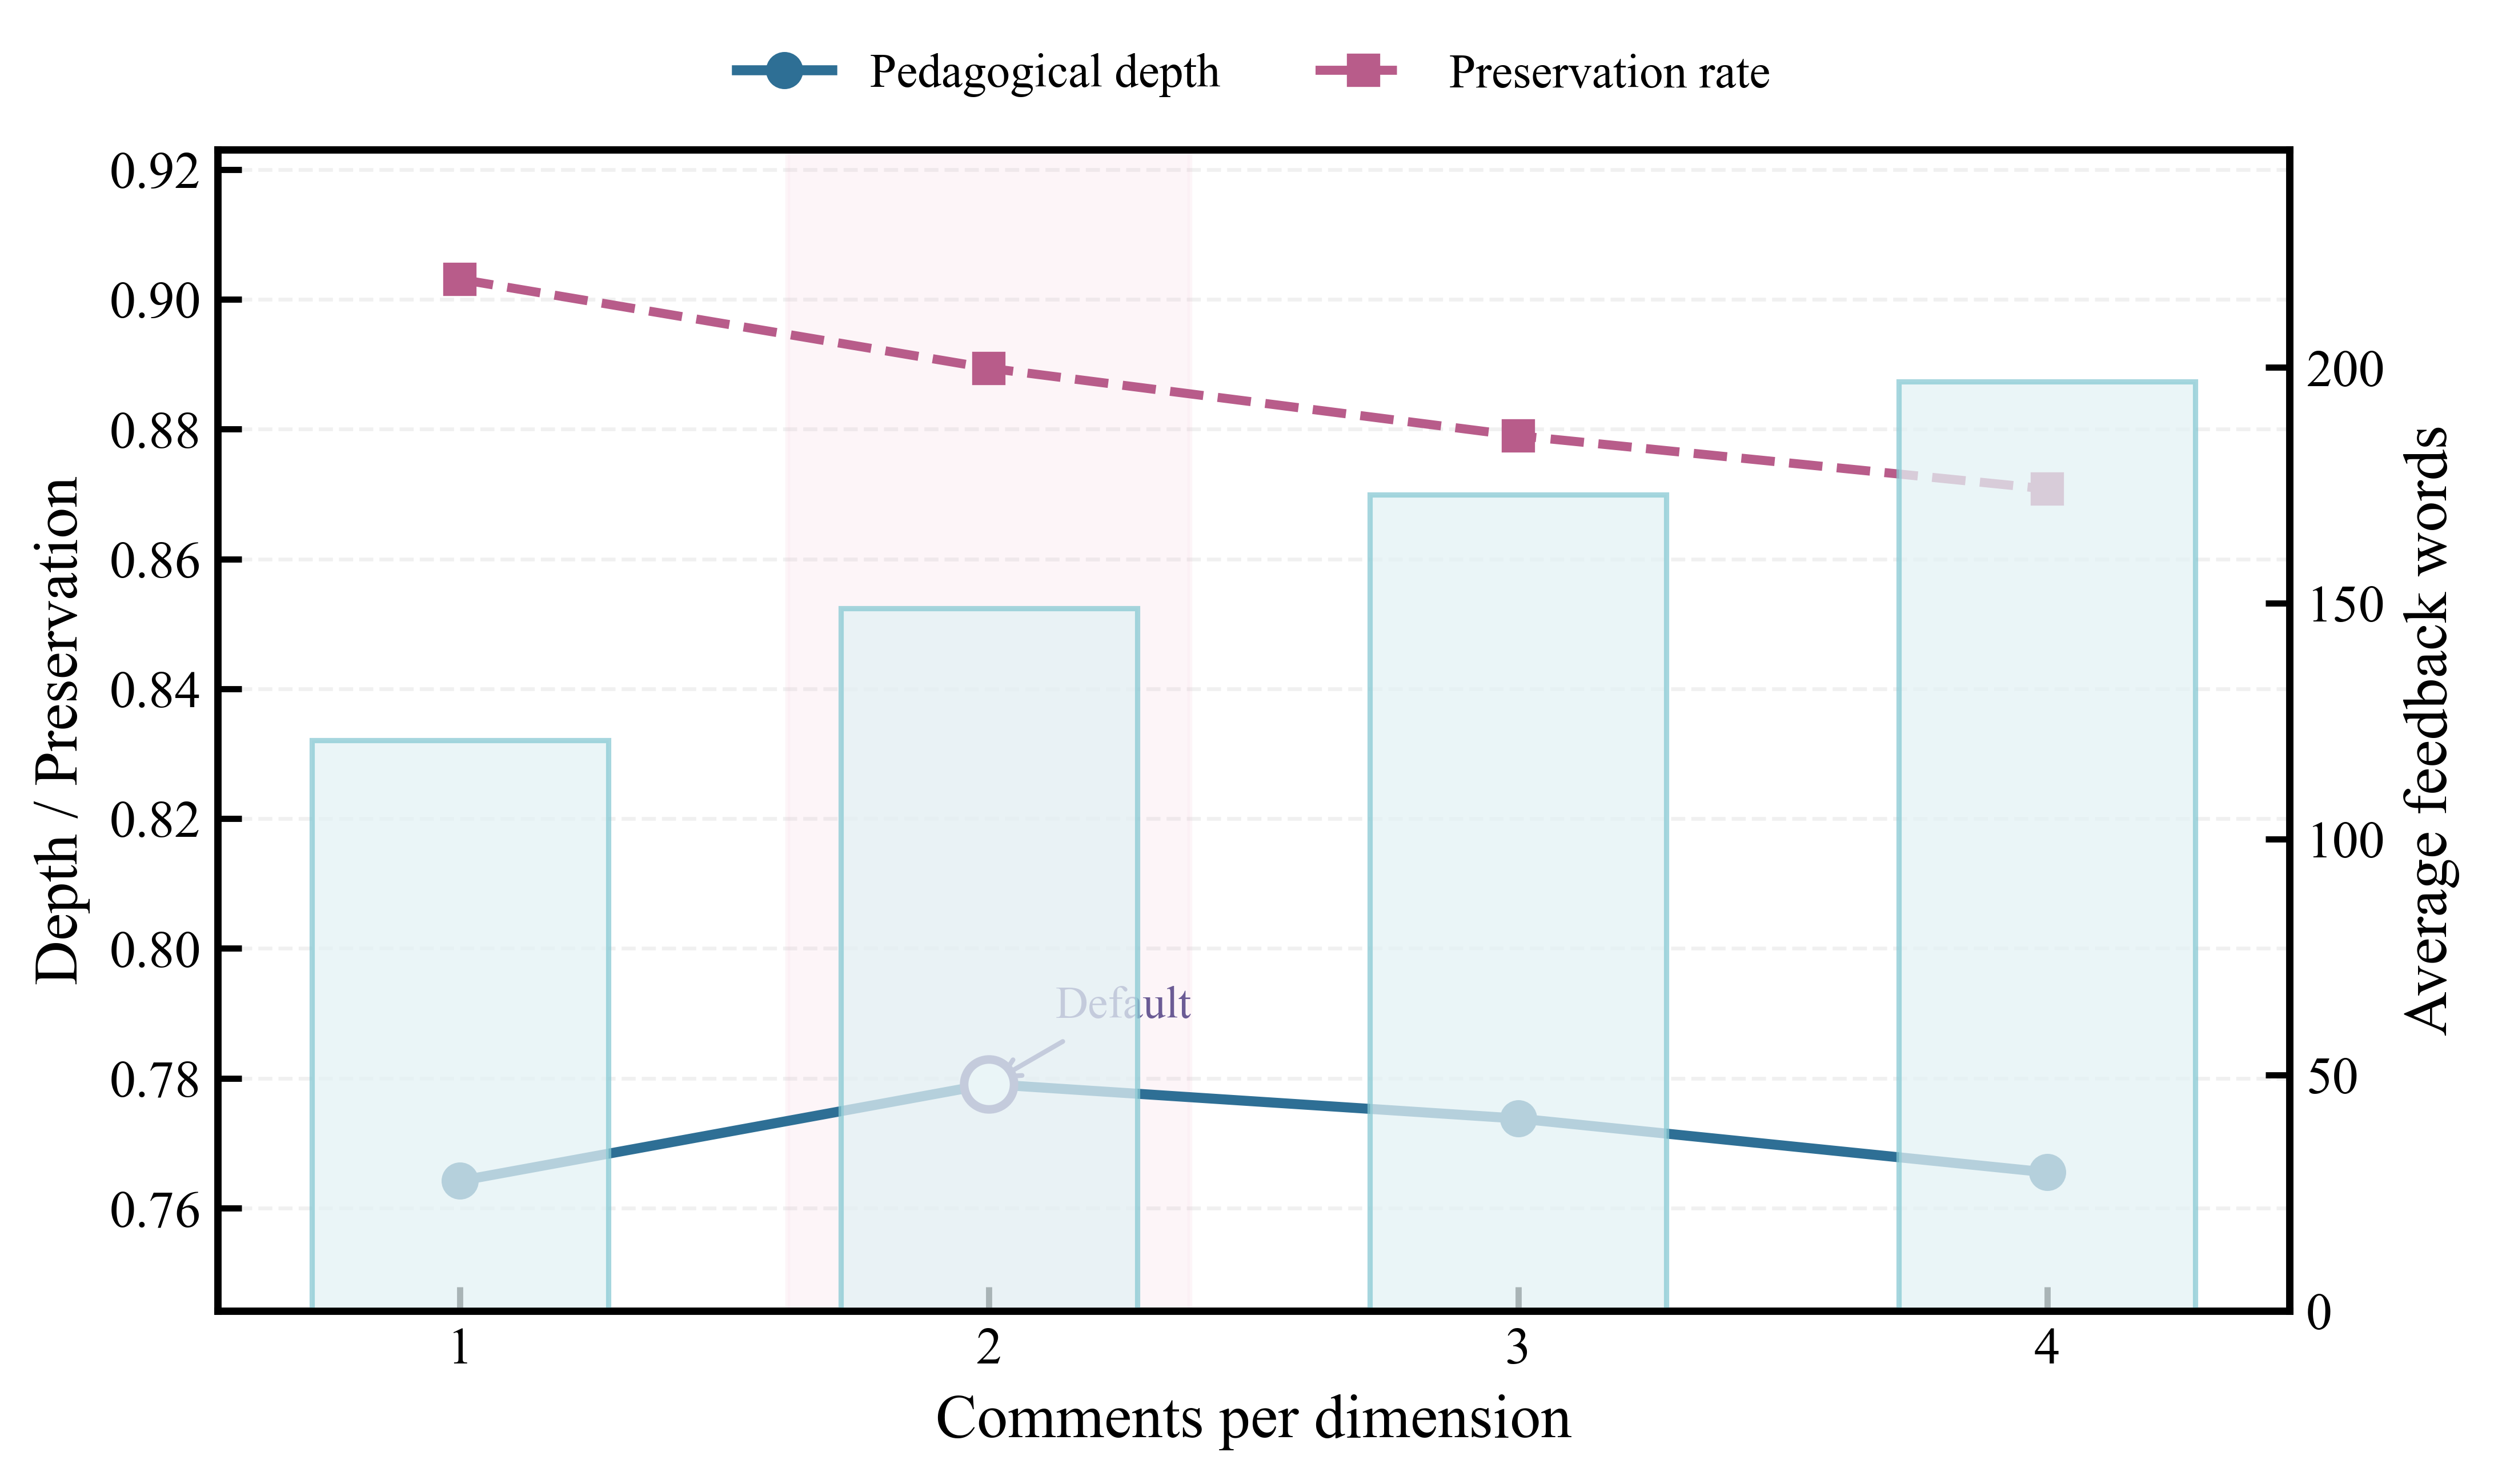
\includegraphics[width=\textwidth]{Fig/hyperparam_3_sensitivity.png}
\end{minipage}
\caption{Combined hyperparameter sensitivity analysis for the representative \textit{Hybrid} setting. From left to right, the panels report the exemplar ratio cap, the maximum number of issue clusters, and the per-dimension comment budget. In each panel, pedagogical depth and student-text preservation rate are shown on the left axis and the auxiliary control indicator on the right axis. Across all three sweeps, the default setting occupies the most favorable part of the performance--control trade-off.}
\label{fig:hyper_sensitivity_all}
\end{figure*}

\subsection{Ablation Studies}

We next study component contributions under the same representative \texttt{GPT-5.4-mini} setting. The ablation design targets staged pedagogical scaffolding, rule grounding, strict exemplar control, and artifact-aware filtering while holding the data split, prompt family, and output budget fixed.

\begin{table}[t]
\centering
\small
\caption{Ablation results for the representative \texttt{GPT-5.4-mini} \textit{Hybrid} setting, averaged over ELL and ASAP. Higher values are better for all reported metrics.}
\label{tab:ablation_main}
\begin{tabularx}{\linewidth}{@{}Yccccc@{}}
\toprule
Variant & Ped.\ depth & $\Delta$Depth & Coverage & Preservation & Schema validity \\
\midrule
Full \textit{Hybrid} & 0.7791 & 0.0000 & 0.9688 & 0.8894 & 0.9942 \\
w/o staged scaffold & 0.7382 & -0.0409 & 0.9254 & 0.8687 & 0.9896 \\
w/o rule grounding & 0.7534 & -0.0257 & 0.9536 & 0.8841 & 0.9924 \\
w/o strict exemplar control & 0.7684 & -0.0107 & 0.9647 & 0.8448 & 0.9940 \\
w/o artifact-aware filtering & 0.7626 & -0.0165 & 0.9591 & 0.8782 & 0.9848 \\
\bottomrule
\end{tabularx}
\end{table}

\begin{figure*}[t]
\centering
\begin{minipage}[t]{0.60\textwidth}
    \centering
    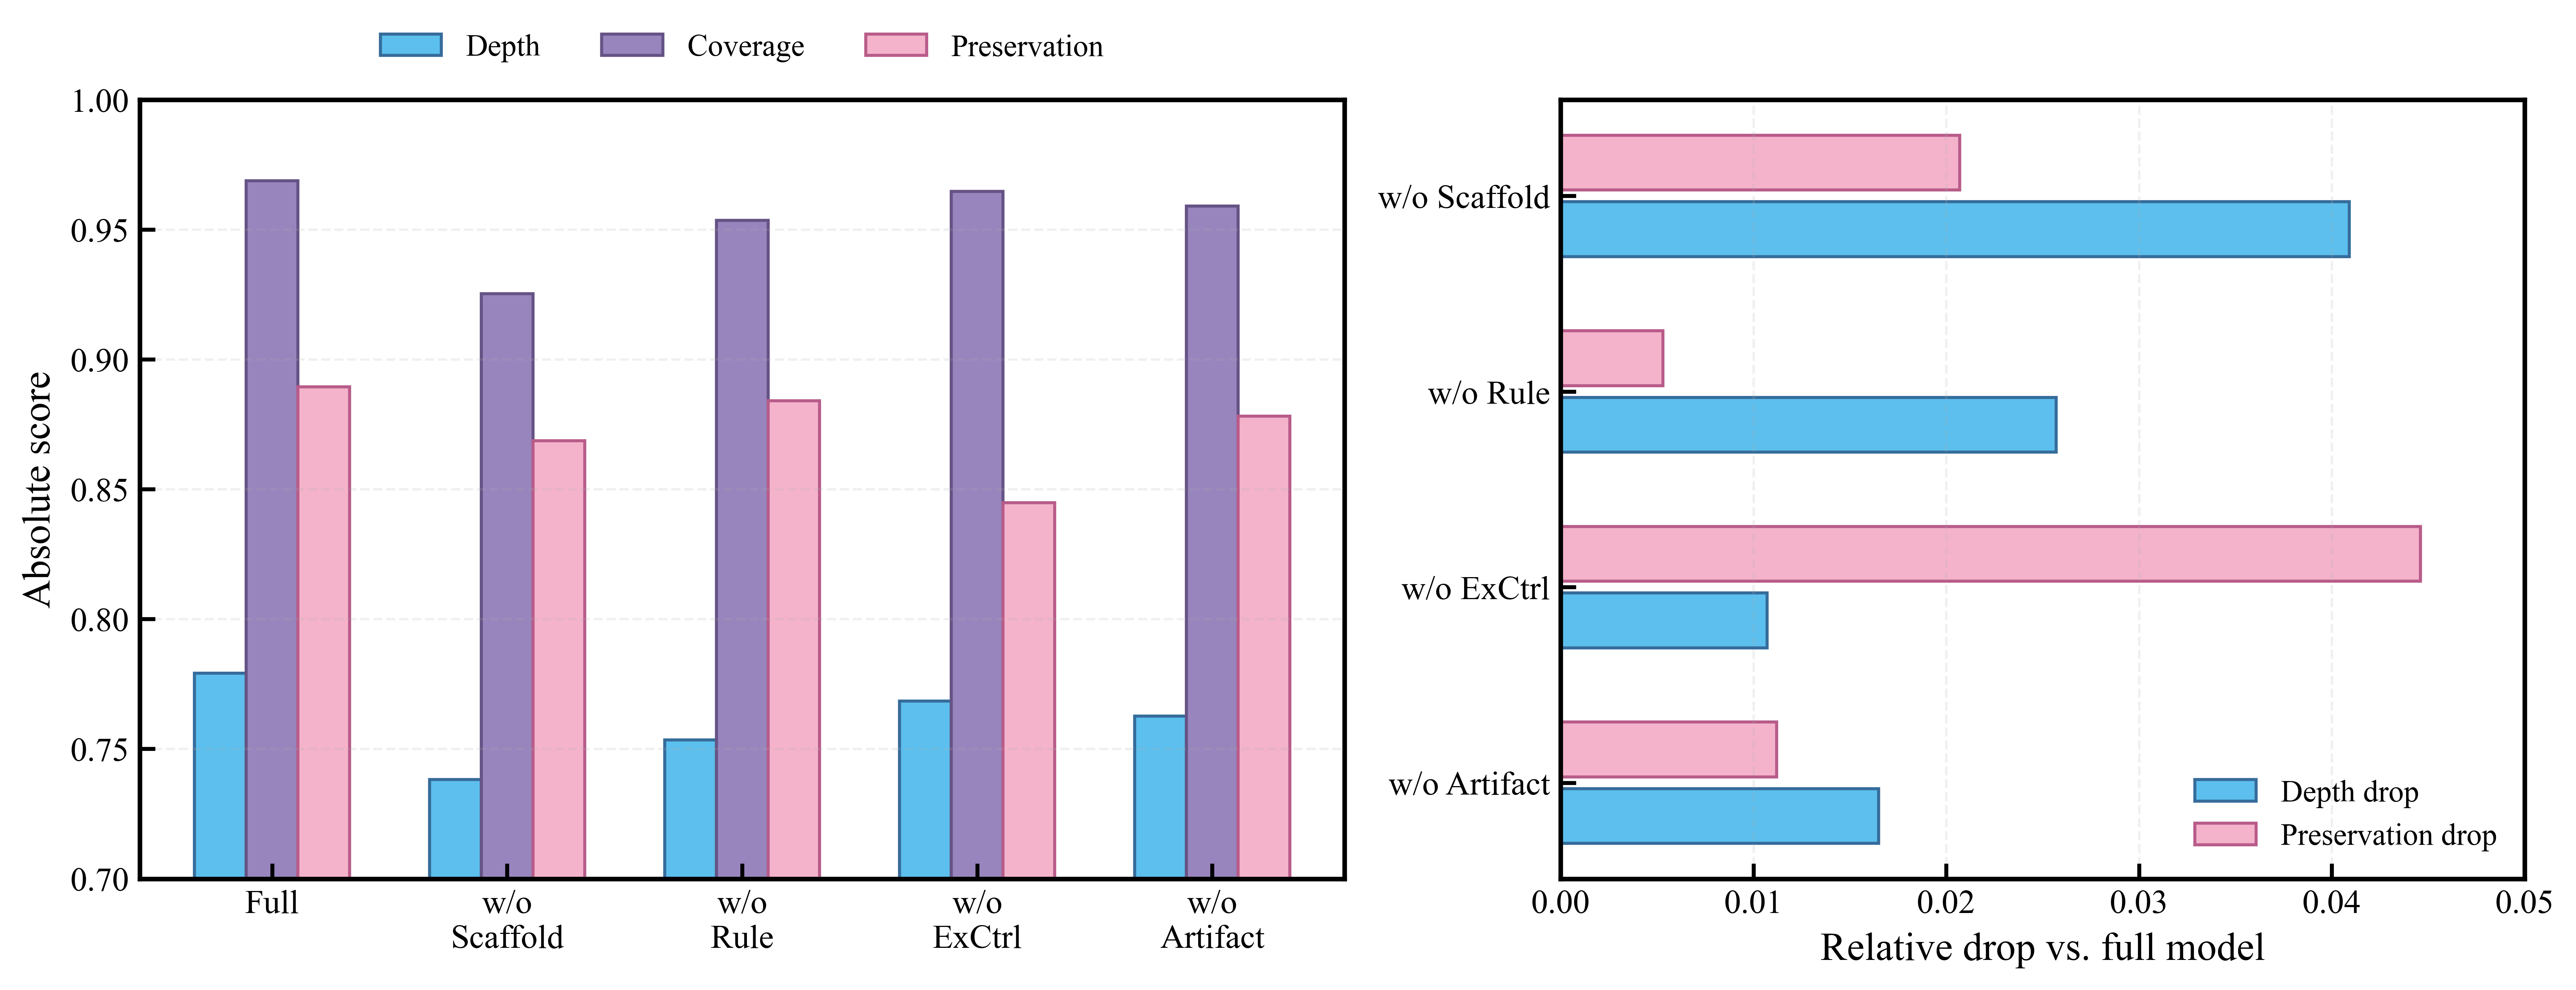
\includegraphics[width=\textwidth]{Fig/ablation_overview.png}
\end{minipage}\hfill
\begin{minipage}[t]{0.35\textwidth}
    \centering
    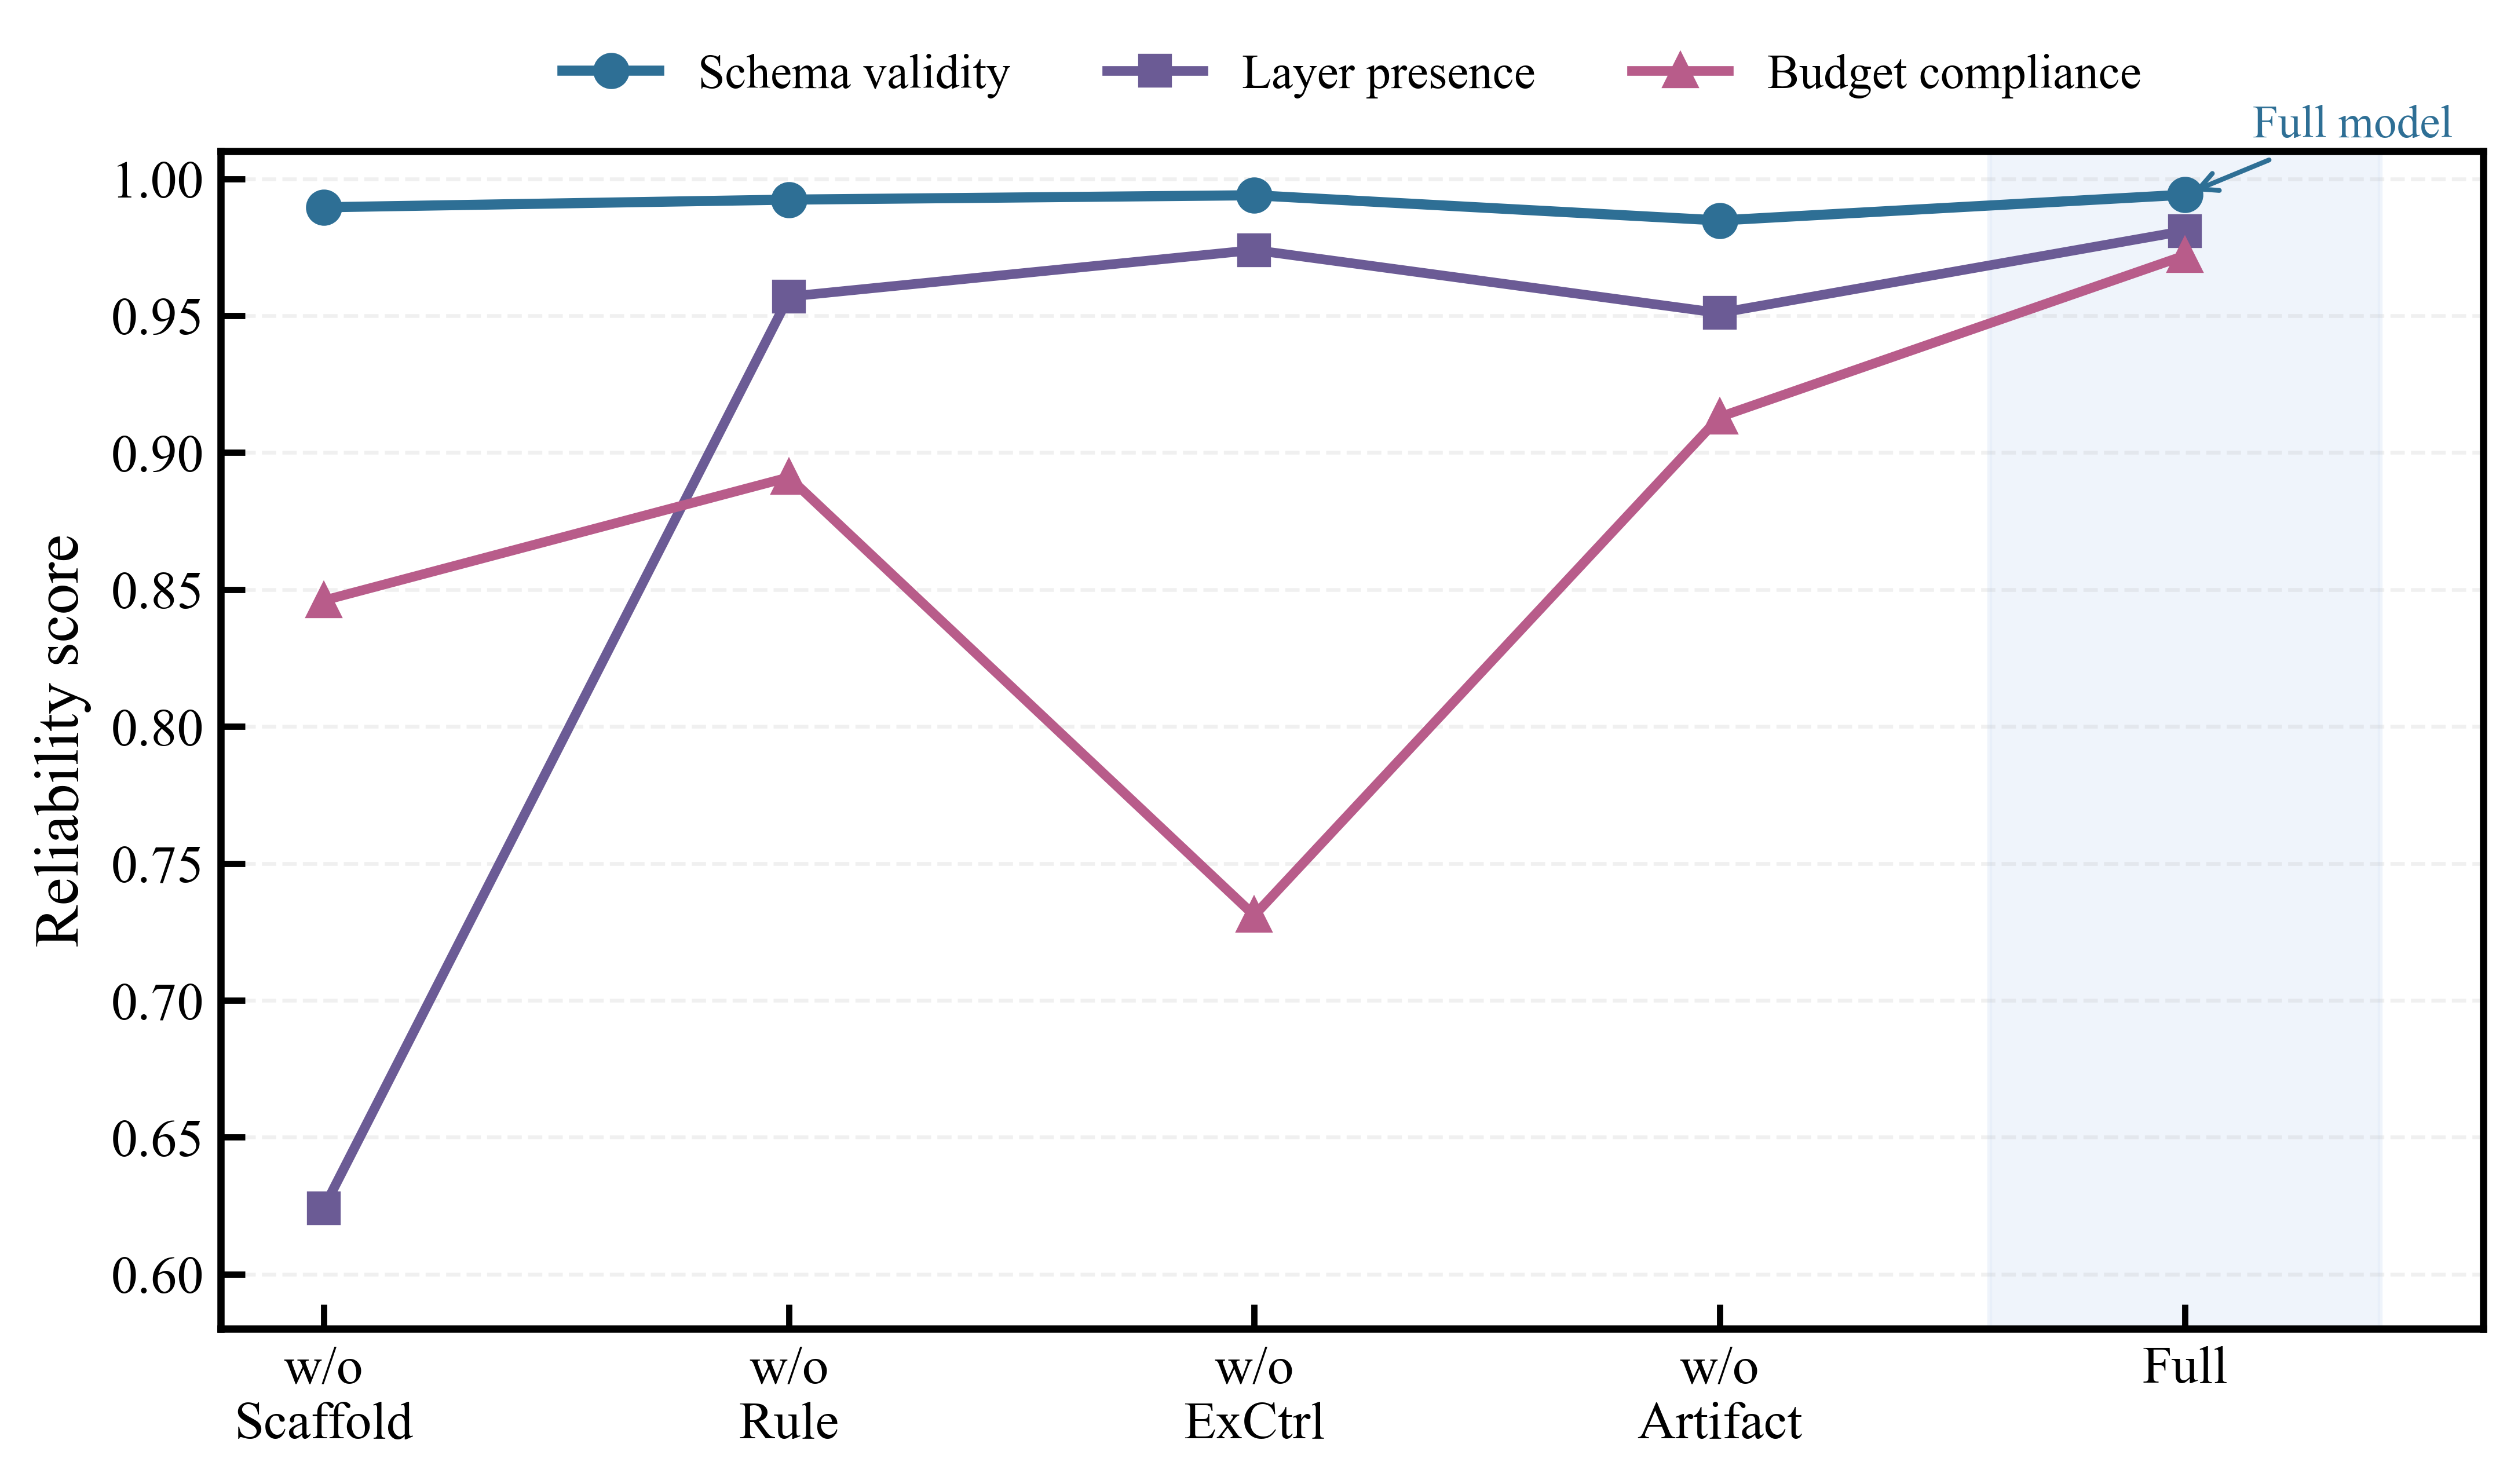
\includegraphics[width=\textwidth]{Fig/reliability_dynamics.png}
\end{minipage}
\caption{Combined ablation summary for the representative \texttt{GPT-5.4-mini} \textit{Hybrid} setting. The left composite plot reports absolute pedagogical depth, dimension coverage, and preservation together with relative drops against the full model, while the right plot reports the reliability profile in terms of schema validity, layer presence, and exemplar-budget compliance.}
\label{fig:ablation_overview}
\end{figure*}

\end{document}
